\chapter{Numerical Solution}
\label{chap:model_soln}
\index{Numerical Solution%
@\emph{Numerical Solution}}%



%\pagestyle{empty}


When solving for the full transition path, we solve the model in two steps.  First, we solve for the steady state prices and allocations.  Next, we iterate backwards solving for prices and allocations along the transition path to the steady state.  Here we define the solution to the model, starting with the steady-state solution.


\section{Solving for stationary steady-state equilibrium}\label{AppSSsolve}

  This section describes the solution method for the stationary steady-state equilibrium described in Definition \ref{DefEquilSS}.  To obtain the steady-state equilibrium, we do the following:
  
 
   \begin{enumerate}
    \item Use the techniques in Chapter \ref{AppPopGrowth} to solve for the steady-state population distribution vector $\bm{\bar{\omega}}$ of the exogenous population process.
    \item Choose an initial guess for the stationary steady-state wage rate, $\bar{w}$ and real interest rate, $\bar{r}$.
%      \begin{itemize}
%        \item A good first guess is a large positive number for all the $\bar{n}_{j,s}$ that is slightly less than $\tilde{l}$ and to choose some small positive number for $\bar{b}_{j,s+1}$ that is small enough to be less than the minimum income that an individual might have $\bar{w}e_{j,s}\bar{n}_{j,s}$.
%      \end{itemize}
   \item With $\bar{w}$ and $\bar{r}$, use an unconstrained root finder to solve the $4\times 2 \times M$ equations defining the steady-state version of the firms' problem.  This will yield $\bar{I}_{m,c}$, $\bar{EL}_{m,c}$, $\bar{V}_{m,c}$, $\bar{p}_{m,c}$.
   \item Using $\bar{p}_{m,c}$ and the fixed coefficient matrix $\Pi$, we can determine $\bar{p}_{i}$, the price of consumption goods.
   \item $\bar{p}_{i}$ and maximization of the consumer's subutility function imply $\bar{p}_{s}$, the price of the composite consumption good.
    \item Perform an unconstrained root finder that chooses $\bar{c}_{j,s}$ and $\bar{b}_{j,s+1}$ that solves the $2JS$ stationary steady-state Euler equations.
    \item Make sure none of the implied steady-state consumptions $\bar{c}_{j,s}+\sum_{i=1}^{I}c_{i,s}$ exceeds income.
      \begin{itemize}
        \item If consumption exceeds income, the individual can not afford the minimum required consumption amounts.  We then...
      \end{itemize}
    \item Given consumption demand and the fixed coefficient matrix $\Xi$, find the implied demand for output, $X_{m}$.
    \item Use the consumer's subutility function over corporate and non-corporate goods to determine demand for corporate and non-corporate production goods to get $X_{m,n}$ and $X_{m,nc}$.
    \item Make sure that demand for these production goods matches the supply given firm's decisions in (iii).
    \item Make sure that none of the Euler errors is too large in absolute value for interior stationary steady-state values. A steady-state Euler error is the following, which is supposed to be close to zero for all $j$ and $s$:
      \begin{align}
        \begin{split}
          &\frac{\chi^n_{s}\left(\frac{b}{\tilde{l}}\right)\left(\frac{\bar{n}_{j,s}}{\tilde{l}}\right)^{v-1}\left[1 - \left(\frac{\bar{n}_{j,s}}{\tilde{l}}\right)\right]^{\frac{1-v}{v}}}{(\bar{c}_{j,s})^{-\sigma}\left(\bar{w} e_{j,s} - \frac{\partial\bar{T}_{j,s}}{\partial \bar{n}_{j,s}}\right)} - 1 \\
          &\qquad\qquad\qquad\qquad\qquad\qquad\qquad\forall j\quad\text{and}\quad E+1\leq s\leq E+S
        \end{split} \label{EqSSeulerrLab} \\
        \begin{split}
          &\frac{e^{-g_y\sigma}\left(\rho_s\chi^b \left(\bar{b}_{j,s+1}\right)^{-\sigma} + \beta(1-\rho_s)(\bar{c}_{j,s+1})^{-\sigma}\left[(1 + \bar{r}) - \frac{\partial \bar{T}_{j,s+1}}{\partial \bar{b}_{j,s+1}}\right]\right)}{(\bar{c}_{j,s})^{-\sigma}} - 1 \\
          &\qquad\qquad\qquad\qquad\qquad\qquad\qquad\forall j \quad\text{and}\quad E+1\leq s\leq E+S-1 \\
        \end{split} \label{EqSSeulerrSav} \\
        &\frac{\chi^b e^{-g_y\sigma}(\bar{b}_{j,E+S+1})^{-\sigma}}{\left(\bar{c}_{j,E+S}\right)^{-\sigma}} - 1 \quad\forall j \label{EqSSeulerrBeq}
      \end{align}
  \end{enumerate}
  
   

%FIRMS STUFF:
%\section{Solving the model}
%
%
%\subsection{Solving for the steady state}
%
%On the supply side (with one sector), we have to solve for the factor prices, $\bar{i}$ and $bar{w}$ (the price of output $\bar{p}^{C}$ is normalized to one), the shadow price of capital, $\bar{q}^{C}$, and the allocations $\bar{EL}^{C}$, $\bar{K}^{C}$, $\bar{I}^{C}$.  From these all the other variables follow trivially.  
%
%Start by solving for the steady-states of Equations \ref{eqn:opt_i} and \ref{eqn:foc_k}.  Equation \ref{eqn:opt_i} becomes:
%
%\begin{equation}
%\label{eqn:opt_i_ss}
%\bar{q}^{C}=\underbrace{1-b^{C}-\bar{\Omega}^{C}\bar{\tau}^{b}(f_{e}-f_{b}b^{C})-f_{d}(1-f_{e})\bar{Z}^{C}}_{\text{function of only parameters}}
%\end{equation}
%
%This yields the solution to $\bar{q}^{C}$.
%
%Next, consider the steady-state of Equation \ref{eqn:foc_k}:
%
%\begin{equation}
%\label{eqn:foc_k_ss}
%\bar{q}^{C}=\frac{1}{1+\bar{\theta}}\left[(1-\delta^{C})\bar{q}^{C} + \frac{\partial \bar{X}^{C}}{\partial \bar{K}^{C}} - \{(1-\bar{\tau}^{b})\bar{\Omega}^{C}\bar{\tau}^{pC} + (1-f_{i}\bar{\tau}^{i})\bar{i}\bar{\Omega}^{C}b^{C} - \delta^{C}(1-b^{C}-\bar{\Omega}^{C}(1-f_{p}\bar{\tau}^{b}b^{C}))\}\right]
%\end{equation}
%
%We can rearrange this and solve for the steady-state marginal product of capital in sector $C$:
%
%\begin{equation}
%\label{eqn:mpk_ss}
%\frac{\partial \bar{X}^{C}}{\partial \bar{K}^{C}} = (\bar{\theta}+\delta^{C})\bar{q}^{C} + (1-\bar{\tau}^{b})\bar{\Omega}^{C}\bar{\tau}^{pC} + (1-f_{i}\bar{\tau}^{i})\bar{i}\bar{\Omega}^{C}b^{C} - \delta^{C}(1-b^{C}-\bar{\Omega}^{C}(1-f_{p}\bar{\tau}^{b}b^{C}))
%\end{equation}
%
%Notice that given Equation \ref{eqn:opt_i_ss}, the RHS to the above equation is function of parameters and the steady state nominal interest rate, $\bar{i}$.  The LHS of the equation is a function of $\bar{K}^{C}$ and $\bar{EL}^{C}$.
%
%I think we can use the following to identify the SS values of the variables of interest:
%\begin{enumerate}
%\item $\bar{i}$ will be determined by the SS of the household's Euler equations (I think this can be done as described in the HH sol'n method)
%\item $\bar{w}$ will be determined by the SS of the household's FOCs for labor supply ((I think this can be done as described in the HH sol'n method)
%\item $\bar{q}^{C}$ is determined by Equation \ref{eqn:opt_i_ss}
%\item $\bar{EL}^{C}$ is determined by the SS version of Equation \ref{eqn:foc_l}, plus $\bar{w}$
%\item $\bar{K}^{C}$ is determined by Equation \ref{eqn:mpk_ss} and $\bar{i}$
%\item $\bar{I}^{C}$ is then solved for using the steady state law of motion for capital $\implies \bar{I}^{C}=\delta^{C}\bar{K}^{C}$
%\end{enumerate}
%
%In solving for $\bar{EL}^{C}$ and $\bar{K}^{C}$, note that we'll have use the MPK and the MPL simultaneously.  Given our production function, we have:
%
%\begin{equation}
%\label{eqn:mpk}
%\frac{\partial X^{C}_{u}}{\partial K^{C}_{u}} = \left[(\gamma_{C})^{1/\epsilon_{C}}(K^{C}_{u})^{(\epsilon_{C}-1)/\epsilon_{C}}+(1-\gamma_{C})^{1/\epsilon_{C}}(EL^{C}_{u})^{(\epsilon_{C}-1)/\epsilon_{C}}\right]^{1/(\epsilon_{C}-1)}(\gamma_{C})^{1/\epsilon_{C}}(K^{C}_{u})^{-1/\epsilon_{C}}
%\end{equation}
%
%and 
%
%\begin{equation}
%\label{eqn:mpl}
%\frac{\partial X^{C}_{u}}{\partial EL^{C}_{u}} = \left[(\gamma_{C})^{1/\epsilon_{C}}(K^{C}_{u})^{(\epsilon_{C}-1)/\epsilon_{C}}+(1-\gamma_{C})^{1/\epsilon_{C}}(EL^{C}_{u})^{(\epsilon_{C}-1)/\epsilon_{C}}\right]^{1/(\epsilon_{C}-1)}(1-\gamma_{C})^{1/\epsilon_{C}}(EL^{C}_{u})^{-1/\epsilon_{C}}
%\end{equation}
%
%We know that, at an optimum, the marginal revenue product of labor equals the wage rate, and the marginal revenue product of capital equals a function of the interest rate, marginal $q$, and the model parameters.  Call this function $g(i_{u},q^{C}_{u},q^{C}_{u-1},\Theta)$.  We thus have $p^{C}_{u}\frac{\partial X^{C}_{u}}{\partial EL^{C}_{u}} =w_{u}$ and $p^{C}_{u}\frac{\partial X^{C}_{u}}{\partial K^{C}_{u}}=g(i_{u},q^{C}_{u},q^{C}_{u-1},\Theta)$.  Dividing these two equations, we have:
%
%\begin{equation}
%\label{eqn:cap_lab_ratio}
%\begin{split}
%& \frac{\frac{\partial X^{C}_{u}}{\partial K^{C}_{u}}}{\frac{\partial X^{C}_{u}}{\partial EL^{C}_{u}}} =\frac{(\gamma_{C})^{1/\epsilon_{C}}(K^{C}_{u})^{-1/\epsilon_{C}}}{(1-\gamma_{C})^{1/\epsilon_{C}}(EL^{C}_{u})^{-1/\epsilon_{C}}}-=\frac{g(i_{u},q^{C}_{u},q^{C}_{u-1},\Theta)}{w_{u}} \\
%& \implies \frac{K^{C}_{u}}{EL^{C}_{u}} =\frac{(1-\gamma_{C})}{\gamma_{C}}\left(\frac{w_{u}} {g(i_{u},q^{C}_{u},q^{C}_{u-1},\Theta)}\right)^{\epsilon_{C}} \\
%\end{split}
%\end{equation}
%
%We can use the SS version of Equation \ref{eqn:cap_lab_ratio} to solve for capital as function of labor (and $\bar{q}, \bar{i}, \bar{w}$), and then use that in the SS version of Equation \ref{eqn:mpl} to solve for labor as s function of $\bar{q}, \bar{i}, \bar{w}$.  We then go back to the SS version of Equation \ref{eqn:cap_lab_ratio} to get the SS choice of capital as a function of $\bar{q}, \bar{i}, \bar{w}$.
%
%All of the above will work for each sector in a model with any number of sectors (though care has to be taken to include the prices of output and capital in those other sectors, since only one sector's output can be the numeraire).
%
%\subsection{Solving for the transition path}
%
%I believe we can just use the Euler equations to go backwards in time, from the SS back along the transition path to $t=0$.  Assume period $T$ is the SS,  The solution would look like the following:
%
%\begin{enumerate}
%\item Use Equation \ref{eqn:foc_k} to solve for the for $q^{C}_{T-1}$ since we have the solution to the RHS of the equation after we've solved for the SS.
%\item Use the law of motion for capital to find: $K^{C}_{T-1}=\frac{K^{C}_{T}-I^{C}_{T-1}}{(1-\delta^{C})}=\frac{\bar{K}^{C}-I^{C}_{T-1}}{(1-\delta^{C})}$
%\item Use Equation \ref{eqn:opt_i} and the value of $q^{C}_{T-1}$ to find $I^{C}_{T-1}$ (and $K^{C}_{T-1}$ given the law of motion relationship.
%\item Given $w_{T-1}$ we can use the FOC for labor demand to find $EL^{C}_{T-1}$
%\item Given $i_{T-1}$ we can use Equation \ref{eqn:foc_k} to solve for $q^{C}_{T-2}$ 
%\item We then repeat the above steps until we work back to $t=0$.
%\end{enumerate}
%
%
%
%To solve for any stationary non-steady-state equilibrium time path of the economy from an arbitrary current state to the steady state, we follow the time path iteration (TPI) method of \citet{AuerbachKotlikoff:1987}. Appendix \ref{AppNonSSsolve} details how to solve for the non-steady-state equilibrium time path using the TPI method. The approach is to choose an arbitrary time path for the stationary aggregate capital stock $\hat{K}_t$, stationary aggregate labor $\hat{L}_t$, and total bequests received $\hat{BQ}_{j,t}$ for each type $j$. This initial guess of a path implies arbitrary beliefs that violate the rational expectations requirement. We then solve for households' optimal decisions given the time paths of those variables, which decisions imply new time paths of those variables. We then update the time path as a convex combination of the initial guess and the new implied path. Figure \ref{FigKpathTPI} shows the equilibrium time path of the aggregate capital stock for the calibration described in Table \ref{TabExogVars} for $T=160$ periods starting from an initial distribution of savings in which $b_{j,s,1}=\bm{\bar{\Gamma}}$ for all $j$ and $s$ in the case that no policy experiment takes place. The initial capital stock $\hat{K}_1$ is not at the steady state $\bar{K}$ because the initial population distribution is not at the steady-state.
%
%
%
%

\section{Solving for stationary non-steady-state equilibrium by time path iteration}\label{AppNonSSsolve}

  \setcounter{equation}{0}

  This section outlines the benchmark time path iteration (TPI) method of \citet{AuerbachKotlikoff:1987} for solving the stationary non-steady-state equilibrium transition path of the distribution of savings. TPI finds a fixed point for the transition path of the distribution of capital for a given initial state of the distribution of capital. The idea is that the economy is infinitely lived, even though the agents that make up the economy are not. Rather than recursively solving for equilibrium policy functions by iterating on individual value functions, one must recursively solve for the policy functions by iterating on the entire transition path of the endogenous objects in the economy (see \citet[ch. 17]{StokeyLucas:1989}).

  The key assumption is that the economy will reach the steady-state equilibrium described in Definition \ref{DefEquilSS} in a finite number of periods $T<\infty$ regardless of the initial state. Let $\bm{\hat{\Gamma}}_t$ represent the distribution of stationary savings at time $t$.
  \begin{equation}\tag{\ref{EqSavDist}}
    \bm{\hat{\Gamma}}_t \equiv \Bigl\{\bigl\{\hat{b}_{j,s,t}\bigr\}_{j=1}^J\Bigr\}_{s=E+2}^{E+S+1}, \quad\forall t
  \end{equation}
  In Section \ref{SecMCEqlbm}, we describe how the stationary non-steady-state equilibrium time path of allocations and price is described by functions of the state $\bm{\hat{\Gamma}}_t$ and its law of motion. TPI starts the economy at any initial distribution of savings $\bm{\hat{\Gamma}}_1$ and solves for its equilibrium time path over $T$ periods to the steady-state distribution $\bm{\bar{\Gamma}}_T$.

  The first step is to assume an initial transition path for aggregate stationary capital $\bm{\hat{K}}^i = \left\{\hat{K}_1^i,\hat{K}_2^i,...\hat{K}_T^i\right\}$, aggregate stationary labor $\bm{\hat{L}}^i = \left\{\hat{L}_1^i,\hat{L}_2^i,...\hat{L}_T^i\right\}$, and total bequests received $\bm{\hat{BQ}}_j^i=\{\hat{BQ}_{j,1}^i,\hat{BQ}_{j,2}^i,...\hat{BQ}_{j,T}^i\}$ for each ability type $j$ such that $T$ is sufficiently large to ensure that $\bm{\hat{\Gamma}}_T = \bar{\bm{\Gamma}}$, $\hat{K}_T^i\left(\bm{\Gamma}_T\right)$, $\hat{L}_T^i\left(\bm{\Gamma}_T\right) = \bar{L}\left(\bar{\bm{\Gamma}}\right)$, and $\hat{BQ}_{j,T}^i\left(\bm{\Gamma}_T\right) = \bar{BQ}_j\left(\bar{\bm{\Gamma}}\right)$ for all $t\geq T$. The superscript $i$ is an index for the iteration number. The transition paths for aggregate capital and aggregate labor determine the transition paths for both the real wage $\bm{\hat{w}}^i = \left\{\hat{w}_1^i,\hat{w}_2^i,...\hat{w}_T^i\right\}$ and the real return on investment $\bm{r}^i = \left\{r_1^i,r_2^i,...r_T^i\right\}$. The time paths for the total bequests received also figure in each period's budget constraint and are determined by the distribution of savings and intended bequests.

  The exact initial distribution of capital in the first period $\bm{\hat{\Gamma}}_1$ can be arbitrarily chosen as long as it satisfies the stationary capital market clearing condition \eqref{EqMktClrCapStat}.
  \begin{equation}\label{EqMktClrCapStat1}
    \hat{K}_1 = \frac{1}{1 + \tilde{g}_{n,1}}\sum_{s=E+2}^{E+S+1}\sum_{j=1}^{J}\hat{\omega}_{s-1,0}\lambda_j \hat{b}_{j,s,1}
  \end{equation}
  Simiilarly, each initial value of total bequests received $\hat{BQ}_{j,1}^i$ must be consistent with the initial distribution of capital through the stationary version of \eqref{EqTotBeq}.
  \begin{equation}\label{EqTotBeqStat1}
    \hat{BQ}_{j,1} = \frac{(1+r_1)\lambda_j}{1+\tilde{g}_{n,1}}\sum_{s=E+1}^{E+S}\rho_s\hat{\omega}_{s,0}\hat{b}_{j,s+1,1} \quad\forall j
  \end{equation}
  However, this is not the case with $\hat{L}_1^i$. Its value will be endogenously determined in the same way the $K_2^i$ is. For this reason, a logical initial guess for the time path of aggregate labor is the steady state in every period $L_t^1 = \bar{L}$ for all $1\leq t\leq T$.

  It is easiest to first choose the initial distribution of savings $\bm{\hat{\Gamma}}_1$ and then choose an initial aggregate capital stock $\hat{K}_1^i$ and initial total bequests received $\hat{BQ}_{j,1}^i$ that correspond to that distribution. As mentioned earlier, the only other restrictions on the initial transition paths for aggregate capital, aggregate labor, and total bequests received is that they equal their steady-state levels $\hat{K}_T^i = \bar{K}\left(\bm{\bar{\Gamma}}\right)$, $\hat{L}_T^i = \bar{L}\left(\bm{\bar{\Gamma}}\right)$, and $\hat{BQ}_{j,T}^i = \bar{BQ}_j\left(\bm{\bar{\Gamma}}\right)$ by period $T$. \citet{EvansPhillips:2014} have shown that the initial guess for the aggregate capital stocks $\hat{K}_t^i$ for periods $1<t<T$ can take on almost any positive values satisfying the constraints above and still have the time path iteration converge.

  Given the initial savings distribution $\bm{\hat{\Gamma}}_1$ and the transition paths of aggregate capital $\bm{\hat{K}}^i = \left\{\hat{K}_1^i,\hat{K}_2^i,...\hat{K}_T^i\right\}$, aggregate labor $\bm{\hat{L}}^i = \left\{\hat{L}_1^i,\hat{L}_2^i,...\hat{L}_T^i\right\}$, and total bequests received $\bm{\hat{BQ}}_j^i = \left\{\hat{BQ}_{j,1}^i,\hat{BQ}_{j,2}^i,...\hat{BQ}_{j,T}^i\right\}$, as well as the resulting real wage $\bm{\hat{w}}^i = \left\{\hat{w}_1^i,\hat{w}_2^i,...\hat{w}_T^i\right\}$, and real return to savings $\bm{r}^i = \left\{r_1^i,r_2^i,...r_T^i\right\}$, one can solve for the period-1 optimal labor supply and intended bequests for each type $j$ of $s=E+S$-aged agents in the last period of their lives $n_{j,E+S,1}=\phi_{j,E+S}(\hat{b}_{j,E+S,1},\hat{BQ}_{j,E+S,1},\hat{w}_1,r_1)$ and $\hat{b}_{j,E+S+1,2}=\psi_{j,E+S}(\hat{b}_{j,E+S,1},\hat{BQ}_{j,E+S,1},\hat{w}_1,r_1)$ using his two $s=E+S$ static Euler equations \eqref{EqEulerLabStat} and \eqref{EqEulerSavEpSstat}.
  \begin{equation}\label{EqEulerSlabt1}
    \begin{split}
      &(\hat{c}_{j,E+S,1})^{-\sigma}\Biggl(\hat{w}_1^i e_{j,E+S} - \frac{\partial\hat{T}_{j,E+S,1}}{\partial n_{j,E+S,1}}\Biggr) = ... \\
      &\qquad\qquad\qquad\qquad \chi^n_{E+S}\biggl(\frac{b}{\tilde{l}}\biggr)\biggl(\frac{n_{j,E+S,1}}{\tilde{l}}\biggr)^{v-1}\Biggl[1 - \biggl(\frac{n_{j,E+S,1}}{\tilde{l}}\biggr)\Biggr]^{\frac{1-v}{v}} \quad\forall j \\
      &\quad\text{where}\quad \hat{c}_{j,E+S,1} = ... \\
      &\qquad\qquad\qquad \left(1 + r_1^i\right)\hat{b}_{j,E+S,1} + \hat{w}_1^i e_{j,E+S}n_{j,E+S,1} + \frac{\hat{BQ}_{j,1}}{\lambda_j} - e^{g_y}\hat{b}_{j,E+S+1,2} - \hat{T}_{j,E+S,1} \\
      &\quad\text{and}\quad \frac{\partial \hat{T}_{j,E+S,1}}{\partial n_{j,E+S,1}} = ... \\
      &\qquad\qquad\qquad \hat{w}_1^i e_{j,E+S}\biggl[\tau^I\bigl(F\hat{a}_{j,E+S,1}\bigr) + \frac{\hat{a}_{j,E+S,1}CDF\bigl[2A(F\hat{a}_{j,E+S,1})+B\bigr]}{\bigl[A(F\hat{a}_{j,E+S,1})^2+B(F \hat{a}_{j,E+S,1})+C\bigr]^2} + \tau^P\Biggr]
    \end{split}
  \end{equation}
  \begin{equation}\label{EqEulerSbeqt1}
    (\hat{c}_{j,E+S,1})^{-\sigma} = \chi^b e^{-g_y\sigma}(\hat{b}_{j,E+S+1,2})^{-\sigma} \quad\forall j
  \end{equation}
  Note that this is simply two equations \eqref{EqEulerSlabt1} and \eqref{EqEulerSbeqt1} and two unknowns $n_{j,E+S,1}$ and $\hat{b}_{j,E+S+1,2}$.

  We then solve the problem for all $j$ types of $E+S-1$-aged individuals in period $t=1$, each of which entails labor supply decisions in the current period $n_{j,E+S-1,1}$ and in the next period $n_{j,E+S,2}$, a savings decision in the current period for the next period $\hat{b}_{j,E+S,2}$ and an intended bequest decision in the last period $\hat{b}_{j,E+S+1,3}$. The labor supply decision in the initial period and the savings period in the initial period for the next period for each type $j$ of $E+S-1$-aged individuals are policy functions of the current savings and the total bequests received and prices in this period and the next $\hat{b}_{j,E+S,2} = \psi_{j,E+S-1}(\hat{b}_{j,E+S-1,1},\{\hat{BQ}_{j,t},\hat{w}_t,r_t\}_{t=1}^2)$ and $\hat{n}_{j,E+S-1,1} = \phi_{j,E+S-1}(\hat{b}_{j,E+S-1,1},\{\hat{BQ}_{j,t},\hat{w}_t,r_t\}_{t=1}^2)$. The labor supply and intended bequests decisions in the next period are simply functions of the savings, total bequests received, and prices in that period $\hat{n}_{j,E+S,2} = \phi_{j,E+S}(\hat{b}_{j,E+S,2},\hat{BQ}_{j,2},\hat{w}_2,r_2)$ and $\hat{b}_{j,E+S+1,3} = \psi_{j,E+S}(\hat{b}_{j,E+S,2},\hat{BQ}_{j,2},\hat{w}_2,r_2)$. These four functions are characterized by the following versions of equations \eqref{EqEulerLabStat}, \eqref{EqEulerSavStat}, and \eqref{EqEulerSavEpSstat}.
  \begin{equation}\label{EqEulerSm1labt1}
    \begin{split}
      &(\hat{c}_{j,E+S-1,1})^{-\sigma}\Biggl(\hat{w}_1^i e_{j,E+S-1} - \frac{\partial\hat{T}_{j,E+S-1,1}}{\partial n_{j,E+S-1,1}}\Biggr) = ... \\
      &\qquad\qquad\qquad \chi^n_{E+S-1}\biggl(\frac{b}{\tilde{l}}\biggr)\biggl(\frac{n_{j,E+S-1,1}}{\tilde{l}}\biggr)^{v-1}\Biggl[1 - \biggl(\frac{n_{j,E+S-1,1}}{\tilde{l}}\biggr)\Biggr]^{\frac{1-v}{v}} \quad\forall j
    \end{split}
  \end{equation}
  \begin{equation}\label{EqEulerSm1savt1}
    \begin{split}
      &(\hat{c}_{j,E+S-1,1})^{-\sigma} = ... \\
      &e^{-g_y\sigma}\Biggl(\rho_{E+S-1}\chi^b \bigl(\hat{b}_{j,E+S,2}\bigr)^{-\sigma} + \beta(1-\rho_{E+S-1})(\hat{c}_{j,E+S,2})^{-\sigma}\Biggl[(1 + r_2^i) - \frac{\partial T_{j,E+S,2}}{\partial b_{j,E+S,2}}\Biggr]\Biggr) \\
      &\qquad\qquad\qquad\qquad\qquad\qquad\qquad\qquad\qquad\qquad\qquad\qquad\qquad\qquad\qquad\qquad\forall j \\
      &\qquad\text{where}\quad \frac{\partial T_{j,E+S,2}}{\partial b_{j,E+S,2}} = ...\\
      &\qquad\qquad r_2^i\Biggl(\tau^I(F\hat{a}_{j,E+S,2}) + \frac{F\hat{a}_{j,E+S,2}CD\left[2A(F\hat{a}_{j,E+S,2}) + B\right]}{\left[A(F\hat{a}_{j,E+S,2})^2 + B(F\hat{a}_{j,E+S,2}) + C\right]^2}\Biggr) ... \\
      &\qquad\qquad \tau^W(\hat{b}_{j,E+S,2}) + \frac{\hat{b}_{j,E+S,2}PHM}{\left(H\hat{b}_{j,E+S,2} + M\right)^2}
    \end{split}
  \end{equation}
  \begin{equation}\label{EqEulerSlabt2}
    \begin{split}
      &(\hat{c}_{j,E+S,2})^{-\sigma}\Biggl(\hat{w}_2^i e_{j,E+S} - \frac{\partial\hat{T}_{j,E+S,2}}{\partial n_{j,E+S,2}}\Biggr) = ... \\
      &\qquad\qquad\qquad \chi^n_{E+S}\biggl(\frac{b}{\tilde{l}}\biggr)\biggl(\frac{n_{j,E+S,2}}{\tilde{l}}\biggr)^{v-1}\Biggl[1 - \biggl(\frac{n_{j,E+S,2}}{\tilde{l}}\biggr)\Biggr]^{\frac{1-v}{v}} \quad\forall j
    \end{split}
  \end{equation}
  \begin{equation}\label{EqEulerSsavt2}
    (\hat{c}_{j,E+S,2})^{-\sigma} = \chi^b e^{-g_y\sigma}(\hat{b}_{j,E+S+1,3})^{-\sigma} \quad\forall j
  \end{equation}
  Note that this is four equations \eqref{EqEulerSm1labt1}, \eqref{EqEulerSm1savt1}, \eqref{EqEulerSlabt2}, and \eqref{EqEulerSsavt2} and four unknowns $n_{j,E+S-1,1}$, $\hat{b}_{j,E+S,2}$, $n_{j,E+S,2}$, and $\hat{b}_{j,E+S+1,3}$.

  This process is repeated for every age of household alive in $t=1$ down to the age $s=E+1$ household at time $t=1$. Each of these households $j$ solves the full set of remaining $S-s+1$ labor supply decisions, $S-s$ savings decisions, and one intended bequest decision at the end of life. After the full set of lifetime decisions has been solved for all the households alive at time $t=1$, each ability $j$ household born in period $t\geq 2$ can be solved for, the solution to which is characterized by the following full set of Euler equations analogous to \eqref{EqEulerLabStat}, \eqref{EqEulerSavStat}, and \eqref{EqEulerSavEpSstat}.
  \begin{equation}\label{EqEulerslabt}
    \begin{split}
      &(\hat{c}_{j,s,t})^{-\sigma}\Biggl(\hat{w}_t^i e_{j,s} - \frac{\partial\hat{T}_{j,s,t}}{\partial n_{j,s,t}}\Biggr) =  \chi^n_{s}\biggl(\frac{b}{\tilde{l}}\biggr)\biggl(\frac{n_{j,s,t}}{\tilde{l}}\biggr)^{v-1}\Biggl[1 - \biggl(\frac{n_{j,s,t}}{\tilde{l}}\biggr)\Biggr]^{\frac{1-v}{v}} \\
      &\qquad\qquad\qquad\qquad\qquad\forall j \quad\text{and}\quad E+1\leq s\leq E+S\quad\text{and}\quad t\geq 2
    \end{split}
  \end{equation}

  \begin{equation}\label{EqEulersSavt}
    \begin{split}
      &(\hat{c}_{j,s,t})^{-\sigma} = ... \\
      &e^{-g_y\sigma}\Biggl(\rho_{s}\chi^b \bigl(\hat{b}_{j,s+1,t+1}\bigr)^{-\sigma} + \beta(1-\rho_{s})(\hat{c}_{j,s+1,t+1})^{-\sigma}\Biggl[(1 + r_{t+1}^i) - \frac{\partial T_{j,s+1,t+1}}{\partial b_{j,s+1,t+1}}\Biggr]\Biggr) \\
      &\qquad\qquad\qquad\forall j \quad\text{and}\quad E+1\leq s\leq E+S-1 \quad\text{and}\quad t\geq 2
    \end{split}
  \end{equation}

  \begin{equation}\label{EqEulerSsavt}
    (\hat{c}_{j,E+S,t})^{-\sigma} = \chi^b e^{-g_y\sigma}(\hat{b}_{j,E+S+1,t+1})^{-\sigma} \quad\forall j \quad\text{and}\quad t\geq 2
  \end{equation}
  For each household of ability type $j$ entering the economy in period $t\geq 1$, the entire set of $2S$ lifetime decisions is characterized by the $2S$ equations represented in \eqref{EqEulerslabt}, \eqref{EqEulersSavt}, and \eqref{EqEulerSsavt}.

  We can then solve for the entire lifetime of savings and labor supply decisions for each age $s=1$ individual in periods $t=2,3,...T$. The central part of the schematic diagram in Figure \ref{FigTPIdiag} shows how this process is done in order to solve for the equilibrium time path of the economy from period $t=1$ to $T$. Note that for each full lifetime savings and labor supply path solved for an individual born in period $t\geq 2$, we can solve for the aggregate capital stock and total bequests received implied by those savings decisions $\bm{\hat{K}}^{i'}$ and $\bm{\hat{BQ}}_{j}^{i'}$ and aggregate labor implied by those labor supply decisions $\bm{\hat{L}}^{i'}$.

  \begin{figure}[p]\centering \captionsetup{width=4.0in}
    \caption{\label{FigTPIdiag}\textbf{Diagram of TPI solution method within each iteration for $S=4$ and $J=1$}}
    \fbox{\resizebox{4.2in}{6.0in}{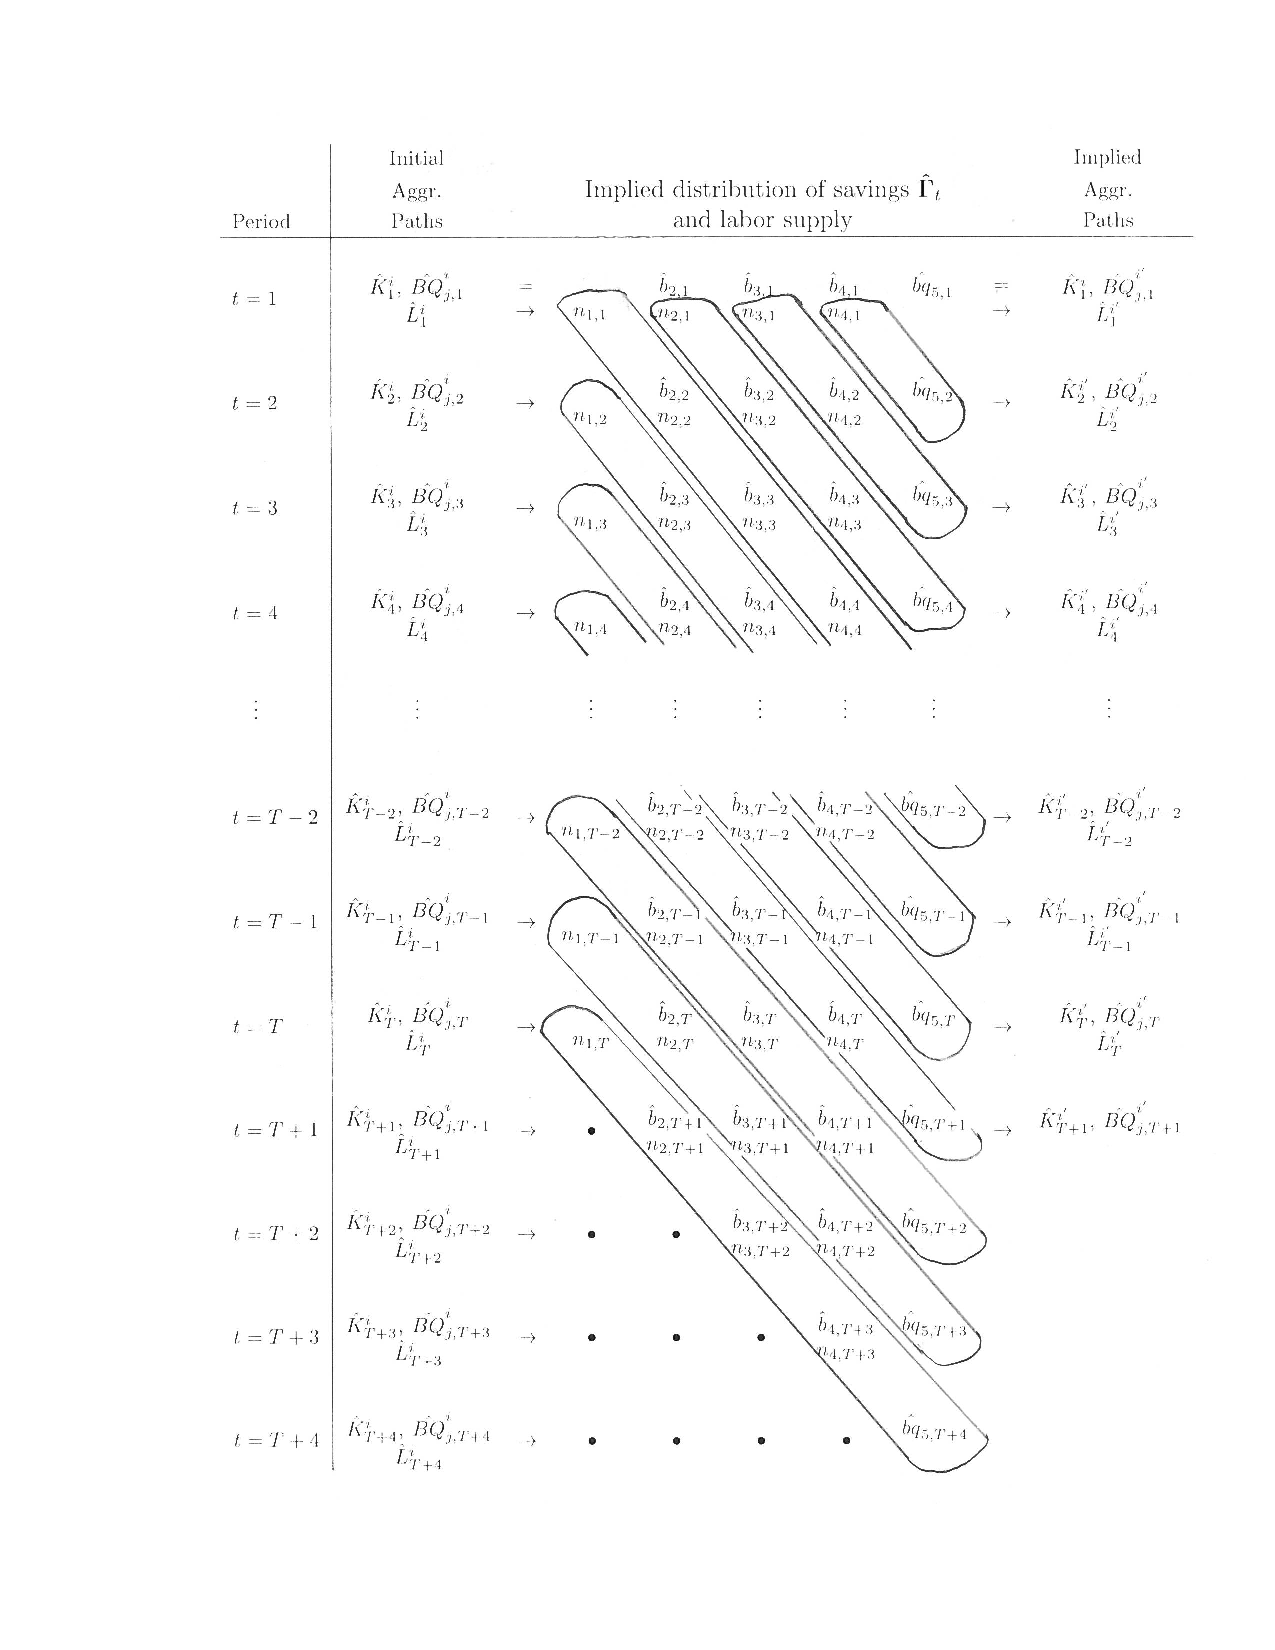
\includegraphics{images/TPIdiag.pdf}}}
  \end{figure}


  % THIS IS THE CODE FOR THE TABLE UNDERLYING THE FIGURE ABOVE
  % \begin{tabular}{>{\footnotesize}l| >{\footnotesize}c >{\footnotesize}c >{\footnotesize}c >{\footnotesize}c >{\footnotesize}c >{\footnotesize}c >{\footnotesize}c >{\footnotesize}c >{\footnotesize}c}
  %          & Initial & & & & & & & & Implied \\
  %          & Aggr. & & \multicolumn{5}{c}{Implied distribution of savings $\bm{\hat{\Gamma}}_t$} & & Aggr. \\
  %   Period & Paths    & & \multicolumn{5}{c}{and labor supply}   & & Paths    \\
  %   \hline
  %   & & & & & & & & & \\
  %   $t=1$ & $\begin{matrix}\hat{K}_1^i, \: \hat{BQ}_{j,1}^i \\ \hat{L}_1^i\end{matrix}$ & $\begin{matrix}= \\ \rightarrow\end{matrix}$ & $\begin{matrix}\: \\ n_{1,1}\end{matrix}$ & $\begin{matrix}\hat{b}_{2,1} \\ n_{2,1}\end{matrix}$ & $\begin{matrix}\hat{b}_{3,1} \\ n_{3,1}\end{matrix}$ & $\begin{matrix}\hat{b}_{4,1} \\ n_{4,1}\end{matrix}$ & $\begin{matrix}\hat{bq}_{5,1} \\ \,\end{matrix}$ & $\begin{matrix}= \\ \rightarrow\end{matrix}$ & $\begin{matrix}\hat{K}_1^i, \: \hat{BQ}_{j,1}^{i'} \\ \hat{L}^{i'}_1\end{matrix}$ \\[10mm]
  %   $t=2$ & $\begin{matrix}\hat{K}_2^i, \: \hat{BQ}_{j,2}^i \\ \hat{L}^i_2\end{matrix}$ & $\rightarrow$ & $\begin{matrix}\: \\ n_{1,2}\end{matrix}$ & $\begin{matrix}\hat{b}_{2,2} \\ n_{2,2}\end{matrix}$ & $\begin{matrix}\hat{b}_{3,2} \\ n_{3,2}\end{matrix}$ & $\begin{matrix}\hat{b}_{4,2} \\ n_{4,2}\end{matrix}$ & $\begin{matrix}\hat{bq}_{5,2} \\ \,\end{matrix}$ & $\rightarrow$ & $\begin{matrix}\hat{K}_2^{i'}, \: \hat{BQ}_{j,2}^{i'} \\ \hat{L}^{i'}_2\end{matrix}$ \\[10mm]
  %   $t=3$ & $\begin{matrix}\hat{K}_3^i, \: \hat{BQ}_{j,3}^i \\ \hat{L}^i_3\end{matrix}$ & $\rightarrow$ & $\begin{matrix}\: \\ n_{1,3}\end{matrix}$ & $\begin{matrix}\hat{b}_{2,3} \\ n_{2,3}\end{matrix}$ & $\begin{matrix}\hat{b}_{3,3} \\ n_{3,3}\end{matrix}$ & $\begin{matrix}\hat{b}_{4,3} \\ n_{4,3}\end{matrix}$ & $\begin{matrix}\hat{bq}_{5,3} \\ \,\end{matrix}$ & $\rightarrow$ & $\begin{matrix}\hat{K}_3^{i'}, \: \hat{BQ}_{j,3}^{i'} \\ \hat{L}^{i'}_3\end{matrix}$ \\[10mm]
  %   $t=4$ & $\begin{matrix}\hat{K}_4^i, \: \hat{BQ}_{j,4}^i \\ \hat{L}^i_4\end{matrix}$ & $\rightarrow$ & $\begin{matrix}\: \\ n_{1,4}\end{matrix}$ & $\begin{matrix}\hat{b}_{2,4} \\ n_{2,4}\end{matrix}$ & $\begin{matrix}\hat{b}_{3,4} \\ n_{3,4}\end{matrix}$ & $\begin{matrix}\hat{b}_{4,4} \\ n_{4,4}\end{matrix}$ & $\begin{matrix}\hat{bq}_{5,4} \\ \,\end{matrix}$ & $\rightarrow$ & $\begin{matrix}\hat{K}_4^{i'}, \: \hat{BQ}_{j,4}^{i'} \\ \hat{L}^{i'}_4\end{matrix}$ \\[10mm]
  %   $\quad\vdots$ & $\vdots$ & & $\vdots$ & $\vdots$ & $\vdots$ & $\vdots$ & $\vdots$ & & $\vdots$ \\[10mm]
  %   $t=T-2$ & $\begin{matrix}\hat{K}_{T-2}^i, \: \hat{BQ}_{j,T-2}^i \\ \hat{L}^i_{T-2}\end{matrix}$ & $\rightarrow$ & $\begin{matrix}\: \\ n_{1,T-2}\end{matrix}$ & $\begin{matrix}\hat{b}_{2,T-2} \\ n_{2,T-2}\end{matrix}$ & $\begin{matrix}\hat{b}_{3,T-2} \\ n_{3,T-2}\end{matrix}$ & $\begin{matrix}\hat{b}_{4,T-2} \\ n_{4,T-2}\end{matrix}$ & $\begin{matrix}\hat{bq}_{5,T-2} \\ \,\end{matrix}$ & $\rightarrow$ & $\begin{matrix}\hat{K}_{T-2}^{i'}, \: \hat{BQ}_{j,T-2}^{i'} \\ \hat{L}^{i'}_{T-2}\end{matrix}$ \\[10mm]
  %   $t=T-1$ & $\begin{matrix}\hat{K}_{T-1}^i, \: \hat{BQ}_{j,T-1}^i \\ \hat{L}^i_{T-1}\end{matrix}$ & $\rightarrow$ & $\begin{matrix}\: \\ n_{1,T-1}\end{matrix}$ & $\begin{matrix}\hat{b}_{2,T-1} \\ n_{2,T-1}\end{matrix}$ & $\begin{matrix}\hat{b}_{3,T-1} \\ n_{3,T-1}\end{matrix}$ & $\begin{matrix}\hat{b}_{4,T-1} \\ n_{4,T-1}\end{matrix}$ & $\begin{matrix}\hat{bq}_{5,T-1} \\ \,\end{matrix}$ & $\rightarrow$ & $\begin{matrix}\hat{K}_{T-1}^{i'}, \: \hat{BQ}_{j,T-1}^{i'} \\ \hat{L}^{i'}_{T-1}\end{matrix}$ \\[10mm]
  %   $t=T$ & $\begin{matrix}\hat{K}_{T}^i, \: \hat{BQ}_{j,T}^i \\ \hat{L}^i_{T}\end{matrix}$ & $\rightarrow$ & $\begin{matrix}\: \\ n_{1,T}\end{matrix}$ & $\begin{matrix}\hat{b}_{2,T} \\ n_{2,T}\end{matrix}$ & $\begin{matrix}\hat{b}_{3,T} \\ n_{3,T}\end{matrix}$ & $\begin{matrix}\hat{b}_{4,T} \\ n_{4,T}\end{matrix}$ & $\begin{matrix}\hat{bq}_{5,T} \\ \,\end{matrix}$ & $\rightarrow$ & $\begin{matrix}\hat{K}_{T}^{i'}, \: \hat{BQ}_{j,T}^{i'} \\ \hat{L}^{i'}_{T}\end{matrix}$ \\[10mm]
  %   $t=T+1$ & $\begin{matrix}\hat{K}_{T+1}^i, \: \hat{BQ}_{j,T+1}^i \\ \hat{L}^i_{T+1}\end{matrix}$ & $\rightarrow$ & $\bullet$ & $\begin{matrix}\hat{b}_{2,T+1} \\ n_{2,T+1}\end{matrix}$ & $\begin{matrix}\hat{b}_{3,T+1} \\ n_{3,T+1}\end{matrix}$ & $\begin{matrix}\hat{b}_{4,T+1} \\ n_{4,T+1}\end{matrix}$ & $\begin{matrix}\hat{bq}_{5,T+1} \\ \,\end{matrix}$ & $\rightarrow$ & $\begin{matrix}\hat{K}_{T+1}^{i'}, \: \hat{BQ}_{j,T+1}^{i'} \\ \:\end{matrix}$ \\[10mm]
  %   $t=T+2$ & $\begin{matrix}\hat{K}_{T+2}^i, \: \hat{BQ}_{j,T+2}^i \\ \hat{L}^i_{T+2}\end{matrix}$ & $\rightarrow$ & $\bullet$ & $\bullet$ & $\begin{matrix}\hat{b}_{3,T+2} \\ n_{3,T+2}\end{matrix}$ & $\begin{matrix}\hat{b}_{4,T+2} \\ n_{4,T+2}\end{matrix}$ & $\begin{matrix}\hat{bq}_{5,T+2} \\ \,\end{matrix}$ & & \\[10mm]
  %   $t=T+3$ & $\begin{matrix}\hat{K}_{T+3}^i, \: \hat{BQ}_{j,T+3}^i \\ \hat{L}^i_{T+3}\end{matrix}$ & $\rightarrow$ & $\bullet$ & $\bullet$ & $\bullet$ & $\begin{matrix}\hat{b}_{4,T+3} \\ n_{4,T+3}\end{matrix}$ & $\begin{matrix}\hat{bq}_{5,T+3} \\ \,\end{matrix}$ & & \\[10mm]
  %   $t=T+4$ & $\begin{matrix}\hat{K}_{T+4}^i, \: \hat{BQ}_{j,T+4}^i \\ \hat{L}^i_{T+4}\end{matrix}$ & $\rightarrow$ & $\bullet$ & $\bullet$ & $\bullet$ & $\bullet$ & $\begin{matrix}\hat{bq}_{5,T+4} \\ \,\end{matrix}$ & & \\
  % \end{tabular}
  % \clearpage

  Once the set of lifetime saving and labor supply decisions has been computed for all individuals alive in $1\leq t\leq T$, we use the household decisions to compute a new implied time path of the aggregate capital stock and aggregate labor. The implied paths of the aggregate capital stock $\bm{\hat{K}}^{i'}=\{\hat{K}_1^i,\hat{K}_2^{i'},...\hat{K}_T^{i'}\}$, aggregate labor $\bm{\hat{L}}^{i'}=\{\hat{L}_1^i,\hat{L}_2^{i'},...\hat{L}_T^{i'}\}$, and total bequests received $\bm{\hat{BQ}}_j^{i'}=\{\hat{BQ}_{j,1}^i,\hat{BQ}_{j,2}^{i'},...\hat{BQ}_{j,T}^{i'}\}$ in general do not equal the initial guessed paths $\bm{\hat{K}}^{i}=\{\hat{K}_1^i,\hat{K}_2^{i},...\hat{K}_T^{i}\}$, $\bm{\hat{L}}^{i}=\{\hat{L}_1^i,\hat{L}_2^{i},...\hat{L}_T^{i}\}$, and $\bm{\hat{BQ}}_j^{i}=\{\hat{BQ}_{j,1}^i,\hat{BQ}_{j,2}^{i},...\hat{BQ}_{j,T}^{i}\}$ used to compute the household savings and labor supply decisions $\bm{\hat{K}}^{i'}\neq\bm{\hat{K}}^i$, $\bm{\hat{L}}^{i'}\neq\bm{\hat{L}}^i$, and $\bm{\hat{BQ}}_j^{i'}\neq\bm{\hat{BQ}}_j^i$.

  Let $\norm{\:\cdot\:}$ be a norm on the space of time paths of the aggregate capital stock $\bm{\hat{K}}\in\mathcal{K}\subset\mathbb{R}_{++}^T$, aggregate labor supply $\bm{\hat{L}}\in\mathcal{L}\subset\mathbb{R}_{++}^T$, and $J$ paths of total bequests received $\bm{\hat{BQ}}_j\in\mathcal{B}\subset\mathbb{R}_{++}^T$. Then the fixed point necessary for the equilibrium transition path from Definition \ref{DefEquilNonSS} has been found when the distance between these $J+2$ paths is arbitrarily close to zero.
  \begin{equation}\label{EqTPIconverge}
    \norm{\Bigl[\bm{\hat{K}}^{i'}, \bm{\hat{L}}^{i'},\bigl\{\bm{\hat{BQ}}_j^{i'}\bigr\}_{j=1}^J\Bigr] - \Bigl[\bm{\hat{K}}^{i},\bm{\hat{L}}^{i},\bigl\{\bm{\hat{BQ}}_j^{i}\bigr\}_{j=1}^J\Bigr]} \leq \ve \quad\text{for}\quad \ve>0
  \end{equation}
  If the fixed point has not been found $\norm{\Bigl[\bm{\hat{K}}^{i'}, \bm{\hat{L}}^{i'},\bigl\{\bm{\hat{BQ}}_j^{i'}\bigr\}_{j=1}^J\Bigr] - \Bigl[\bm{\hat{K}}^{i},\bm{\hat{L}}^{i},\bigl\{\bm{\hat{BQ}}_j^{i}\bigr\}_{j=1}^J\Bigr]} > \ve$, then new transition paths for the aggregate capital stock and aggregate labor are generated as a convex combination of $\Bigl[\bm{\hat{K}}^{i'},\bm{\hat{L}}^{i'},\bigl\{\bm{\hat{BQ}}_j^{i'}\bigr\}_{j=1}^J\Bigr]$ and $\Bigl[\bm{\hat{K}}^{i},\bm{\hat{L}}^{i},\bigl\{\bm{\hat{BQ}}_j^{i}\bigr\}_{j=1}^J\Bigr]$.
  \begin{equation}\label{EqTPInewpath}
    \begin{split}
      \bm{\hat{K}}^{i+1} &= \nu\bm{\hat{K}}^{i'} + (1-\nu)\bm{\hat{K}}^{i} \\
      \bm{\hat{L}}^{i+1} &= \nu\bm{\hat{L}}^{i'} + (1-\nu)\bm{\hat{L}}^{i} \\
      \bm{\hat{BQ}}_1^{i+1} &= \nu\bm{\hat{BQ}}_1^{i'} + (1-\nu)\bm{\hat{BQ}}_1^{i} \\
      &\vdots \\
      \bm{\hat{BQ}}_J^{i+1} &= \nu\bm{\hat{BQ}}_J^{i'} + (1-\nu)\bm{\hat{BQ}}_J^{i}
    \end{split} \quad\quad\text{for}\quad \nu\in(0,1]
  \end{equation}
  This process is repeated until the initial transition paths for the aggregate capital stock, aggregate labor, and total bequests received are consistent with the transition paths implied by those beliefs and household and firm optimization.

  In essence, the TPI method iterates on individual beliefs about the time path of prices represented by a time paths for the aggregate capital stock $\bm{\hat{K}}^i$, aggregate labor $\bm{\hat{L}}^i$, and total bequests received $\bm{\hat{BQ}}_j^i$ until a fixed point in beliefs is found that are consistent with the transition paths implied by optimization based on those beliefs.

  The following are the steps for computing a stationary non-steady-state equilibrium time path for the economy.
  \begin{enumerate}
    \item Input all initial parameters. See Table \ref{TabExogVars}.
      \begin{enumerate}
        \item The value for $T$ at which the non-steady-state transition path should have converged to the steady state should be at least as large as the number of periods it takes the population to reach its steady state $\bm{\bar{\omega}}$ as described in Appendix \ref{AppPopGrowth}.
      \end{enumerate}

    \item Choose an initial distribution of savings and intended bequests $\bm{\hat{\Gamma}}_1$ and then calculat the initial state of the stationarized aggregate capital stock $\hat{K}_1$ and total bequests received $\hat{BQ}_{j,1}$ consistent with $\bm{\hat{\Gamma}}_1$ according to \eqref{EqMktClrCapStat} and \eqref{EqTotBeqStat1}.
      \begin{enumerate}
        \item Note that you must have the population weights from the previous period $\hat{\omega}_{s,0}$ and the growth rate between period 0 and period 1 $\tilde{g}_{n,1}$to calculate $\hat{BQ}_{j,1}$.
      \end{enumerate}
    \item Conjecture transition paths for the stationarized aggregate capital stock $\bm{\hat{K}}^1=\{\hat{K}^1_t\}_{t=1}^\infty$, stationarized aggregate labor $\bm{\hat{L}}^1=\{\hat{L}^1_t\}_{t=1}^\infty$, and total bequests received $\bm{\hat{BQ}}_j^1=\{\hat{BQ}^{1}_{j,t}\}_{t=1}^\infty$ where the only requirements are that $\hat{K}^i_1$ and $\hat{BQ}^i_{j,1}$ are functions of the initial distribution of savings $\bm{\hat{\Gamma}}_1$ for all $i$ is your initial state and that $\hat{K}^i_t=\bar{K}$, $\hat{L}^i_t=\bar{L}$, and $\hat{BQ}^i_{j,t}= \bar{BQ}_j$ for all $t\geq T$. The conjectured transition paths of the aggregate capital stock $\bm{\hat{K}}^i$ and aggregate labor $\bm{\hat{L}}^i$ imply specific transition paths for the real wage $\bm{\hat{w}}^i=\{\hat{w}^i_t\}_{t=1}^\infty$ and the real interest rate $\bm{r}^i=\{r^i_t\}_{t=1}^\infty$ through expressions \eqref{EqFOCwageStat} and \eqref{EqFOCrate}.
      \begin{enumerate}
        \item An intuitive choice for the time path of aggregate labor is the steady-state in every period $\hat{L}^1_t = \bar{L}$ for all $t$.
      \end{enumerate}
    \item With the conjectured transition paths $\bm{\hat{w}}^i$, $\bm{r}^i$, and $\bm{\hat{BQ}}_j^i$ one can solve for the lifetime policy functions of each household alive at time $1\leq t\leq T$ using the systems of Euler equations of the form \eqref{EqEulerLabStat}, \eqref{EqEulerSavStat}, and \eqref{EqEulerSavEpSstat} and following the diagram in Figure \ref{FigTPIdiag}.
    \item Use the implied distribution of savings and labor supply in each period (each row of $\hat{b}_{j,s,t}$ and $n_{j,s,t}$ in Figure \ref{FigTPIdiag}) to compute the new implied time paths for the aggregate capital stock $\bm{\hat{K}}^{i'} = \{\hat{K}_1^i,\hat{K}_2^{i'},...\hat{K}_T^{i'}\}$, aggregate labor supply $\bm{\hat{L}}^{i'} = \{\hat{L}_1^i,\hat{L}_2^{i'},...\hat{L}_T^{i'}\}$, and total bequests received $\bm{\hat{BQ}}_j^{i'} = \{\hat{BQ}_{j,1}^i,\hat{BQ}_{j,2}^{i'},...\hat{BQ}_{j,T}^{i'}\}$.
    \item Check the distance between the two sets time paths.
      \begin{equation*}
        \norm{\Bigl[\bm{\hat{K}}^{i'}, \bm{\hat{L}}^{i'},\bigl\{\bm{\hat{BQ}}_j^{i'}\bigr\}_{j=1}^J\Bigr] - \Bigl[\bm{\hat{K}}^{i},\bm{\hat{L}}^{i},\bigl\{\bm{\hat{BQ}}_j^{i}\bigr\}_{j=1}^J\Bigr]}
      \end{equation*}
      \begin{enumerate}
        \item If the distance between the initial time paths and the implied time paths is less-than-or-equal-to some convergence criterion $\ve>0$, then the fixed point has been achieved and the equilibrium time path has been found \eqref{EqTPIconverge}.
        \item If the distance between the initial time paths and the implied time paths is greater than some convergence criterion $\norm{\cdot}>\ve$, then update the guess for the time paths according to \eqref{EqTPInewpath} and repeat steps (4) through (6) until a fixed point is reached.
      \end{enumerate}
  \end{enumerate}

